\documentclass[../stats.tex]{subfiles}
\graphicspath{{\subfix{../figures/}}}
\begin{document}
\chapter{Exploring Two-Variable Data}
\section{Two Categorical Variables}
In Unit 1, we explored how bar graphs are a commonly used way to display categorical data. When we have two categorical variables to compare, we still use bar graphs, but they become a segmented bar plot or a mosaic plot.

Here is data on the breakdown of state locations and how the state voted in the 2020 election.
\begin{center}
    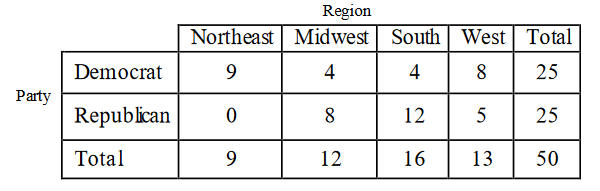
\includegraphics[width=0.8\textwidth]{2.1.1.PNG}
\end{center}

A side by side bar graph merges two bar graphs into one, in an attempt to compare the distributions of the two categorical variables.
\begin{center}
    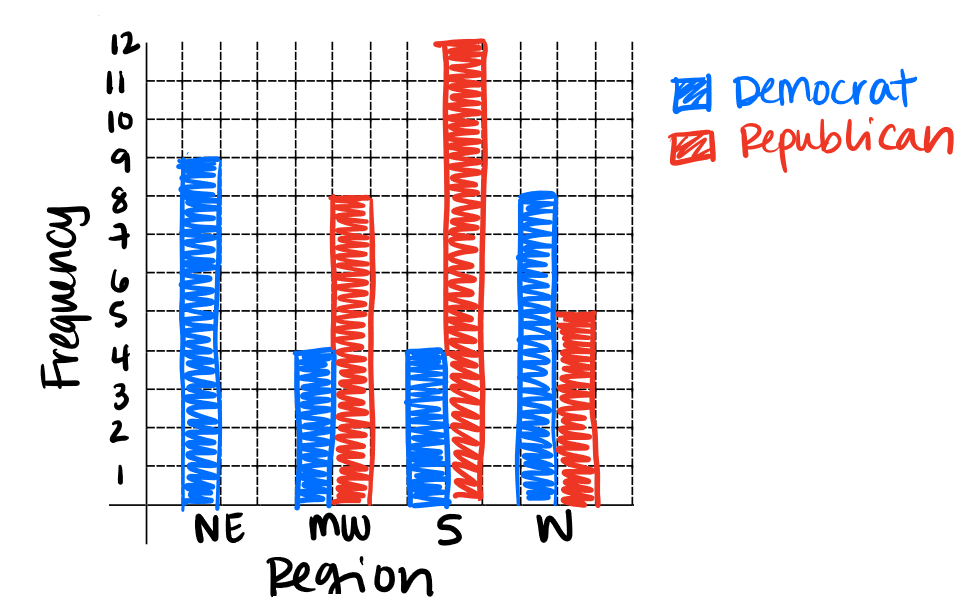
\includegraphics[width=0.8\textwidth]{2.1.2.PNG}
\end{center}

A segmented bar graph is another way to display the data, where each group is split up by its relative frequency.
\begin{center}
    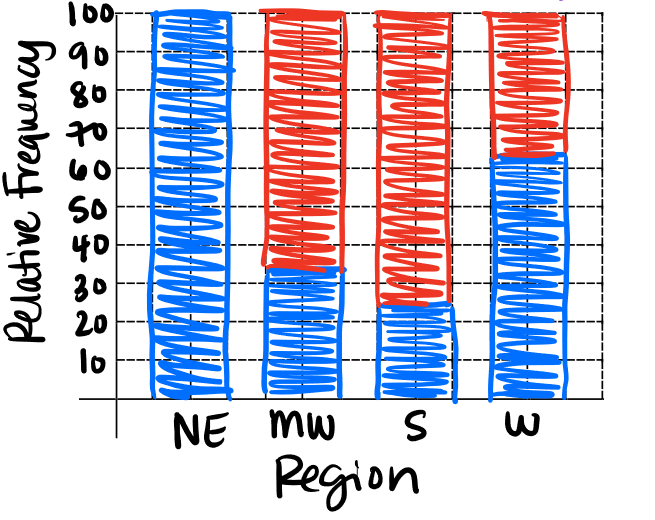
\includegraphics[width=0.8\textwidth]{2.1.3.PNG}
\end{center}

A mosaic plot is similar to a segmented bar graph, but it draws attention to the sizes of each group.
\begin{center}
    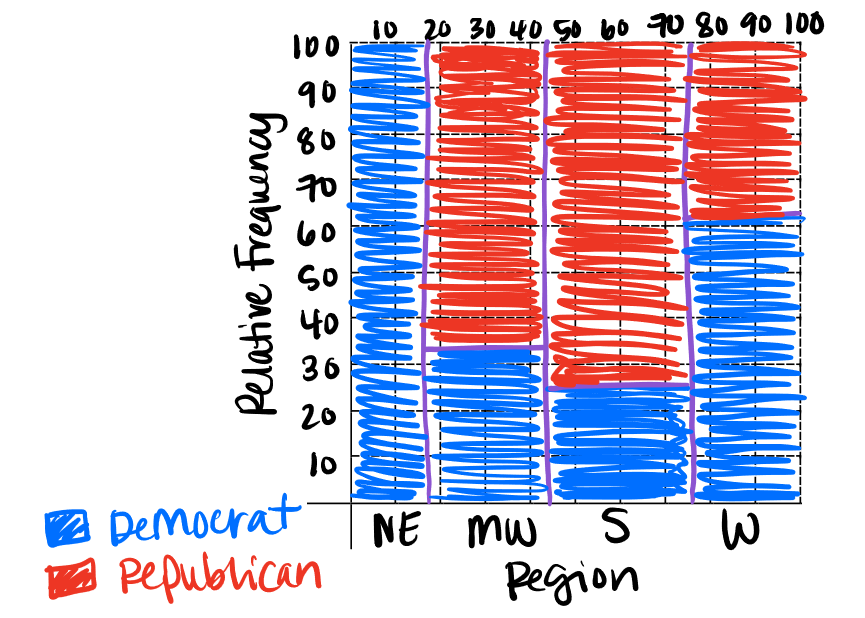
\includegraphics[width=0.8\textwidth]{2.1.4.PNG}
\end{center}

When you are working with two categorical variables, most of the time, the raw data is given in the form of a two way table - it is a table 
listing two categorical variables whose values have been paired. Each set of numbers in a two-way table has a specific name.

Joint relative frequencies: ratio of the frequency in a cell and the total number of data values.

Marginal relative frequencies: ratio of the sum in a row or column and the total number of data values.

Conditional relative frequencies: ratio of a joint relative frequency and related marginal relative frequency.

\begin{example}
    \begin{center}
        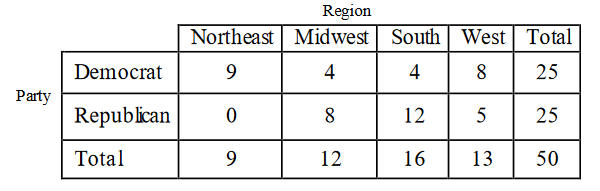
\includegraphics[width=0.8\textwidth]{2.1.1.PNG}
    \end{center}

    Joint Relative Frequency: What are the percent of states that are in the Midwest and voted ``Democrat''? Answer: 8\%

    Marginal Relative Frequency: Percent of states that are in the South. Answer: 32\%

    Conditional Relative Frequency: Of the states that voted ``democrat'', the percent that is from the West. Answer: 32\%
\end{example}

\begin{example}
    The direction of a technical school was curious about whether there is a relationship between students who complete one of the school's 
    most popular health sciences certificate programs and whether those students go on to complete more advanced studies in the health sciences within 
    two years of completing the certificate program. She randomly selected 100 students who completed the program. Data collected on these students is shown in the table below.
    \begin{center}
        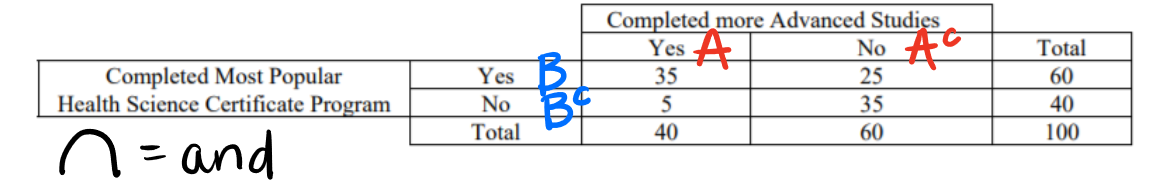
\includegraphics[width=0.8\textwidth]{2.1.5.PNG}
    \end{center}

    Note we are letting A, A$^c$, B and B$^c$ correspond to the 4 different possibilities.

    The four following questions are true or false questions.

    (a) Being a person who completed more advanced studies is more likely than being a person who did not complete more advanced studies.

    False, 40 is not greater than 60.

    (b) Being a person who completed the program is less likely than being a person who did not complete the program.

    False, 60 is greater than 40.

    (c) Being a person who completed the program and completed more advanced studies is less likely than being a person who did not complete the pgoram and did not complete more advanced studies.

    False, 35 is equal to 35.

    (d) Being a person who did not complete the program but completed more advanced studies is less likely than being a person who completed the pgoram and completed more advanced studies.

    True

    (f) Being a person who completed the pgoram but did not complete more advanced studies is more likely than being a person who did not complete the program and did not complete more advanced studies.

    False, 25 is not more than 35.
\end{example}

\begin{example}
    A 1968 sample study among the Pima Indians of Arizona investigated the relationship between a mother's diabetic status and the appearance of birth defects in her children. The results appear in the two-way table below.
    \begin{center}
        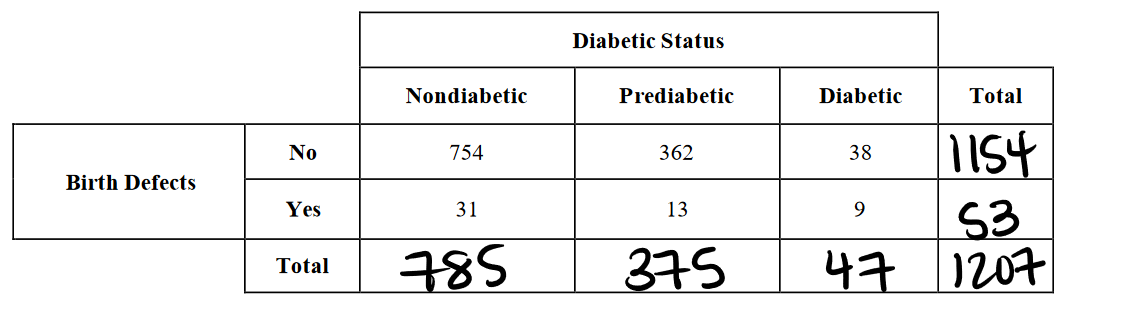
\includegraphics[width=0.8\textwidth]{2.1.6.PNG}
    \end{center}

    (a) Compute the conditional distributions of birth defects for each diabetic status.

    For nondiabetic it is 31/785, for prediabetic it is 13/375, for diabetic it is 9/47.

    (b) Display the conditional distributions in a segmented bar graph. Don't forget to labe your graph completely. Comment on any clear associations you see.
    \begin{center}
        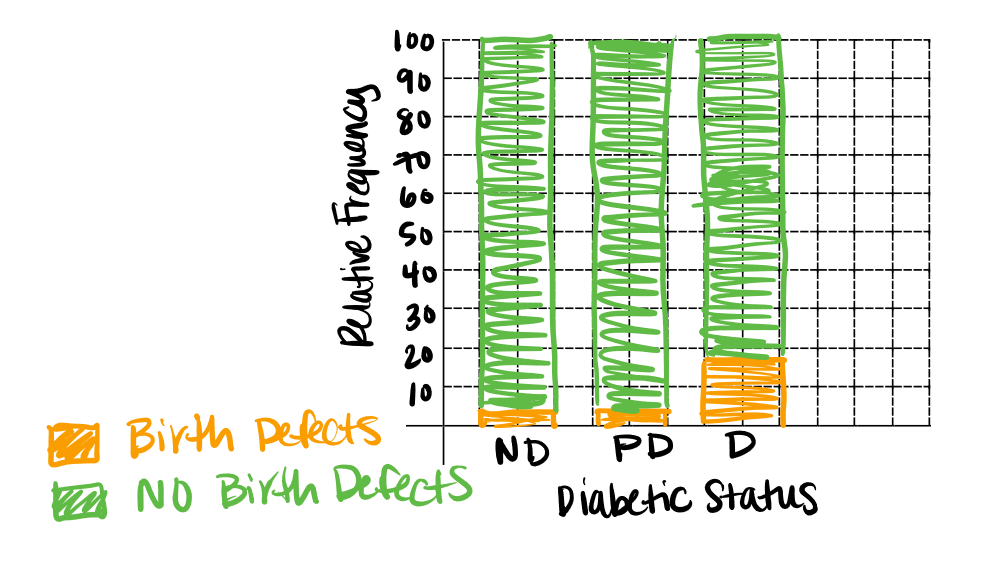
\includegraphics[width=0.8\textwidth]{2.1.7.PNG}
    \end{center}
    There is no association.
\end{example}

\section{Scatterplots and Correlation}
We have worked with data for bar graphs, box plots, dot plots, and histograms. The type of data that is represented with these graphs are univariate data.

When we compare two variables (bivariate data), we are exploring the relationship between them.

Most statistical studies involve more than one variable. Often in the AP Statistics exam, you will be asked to compare 
two data sets by using side by side boxplots or histograms etc. However, there are times where we want to examine relationships among several variables for the same group of data.

When you examine the relationship between two variables you need to start with a scatterplot.

A scatterplot shows the relationship between two quantitative variables measured on the same individuals. The values of one variable appear on the horizontal axis, and the values 
of the other variable appear on the vertical axis. Each individual in the data appears as a point in the plot fixed by the values of both variables for that individual.

Here is a scatterplot representing Arm Span vs Height:

First, we have to identify and name the correct variables used in this study.

A response variable measures the outcome of a study or an observation (y variable, dependent)

An explanatory variable helps explain or influences change in a response variable. (x variable, independent)
\begin{center}
    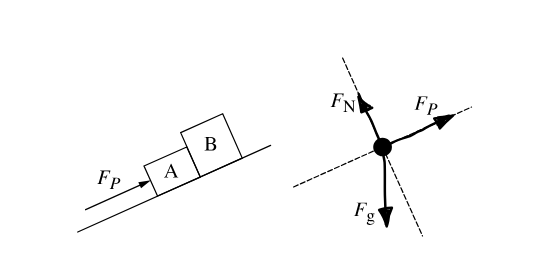
\includegraphics[width=0.8\textwidth]{2.2.1.PNG}
\end{center}
You will often find explanatory variables called independent variables, and reponse variables called dependent variables.
The idea behind this language is that the response variable depends on the explanatory variable.
Because the words independent and dependent have other, unrelated meanings in statistics, we won't use them here.

\begin{itemize}
    \item In any graph of data, look for overall pattern and for striking deviations from that pattern.
    \item You can describe the overall pattern of a scatterplot by the direction, form, and strength of the relationship.
    \item An important kind of deviation is an outlier, and individual value that falls outside the overall pattern of the relationship.
\end{itemize}
Things to look for in a scatterplot:
\begin{itemize}
    \item Form: Overall pattern or deviations from the pattern 
    \item Direction: Positive or negative slope 
    \item Strength: How close do the points lie to a simple form 
\end{itemize}

Examples of form:
\begin{center}
    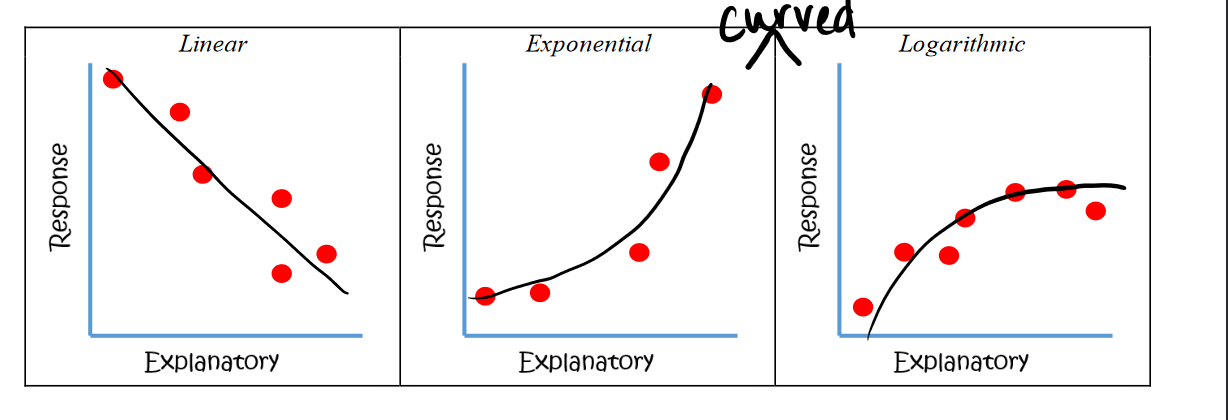
\includegraphics[width=0.8\textwidth]{2.2.2.PNG}
\end{center}

Examples of direction:
\begin{center}
    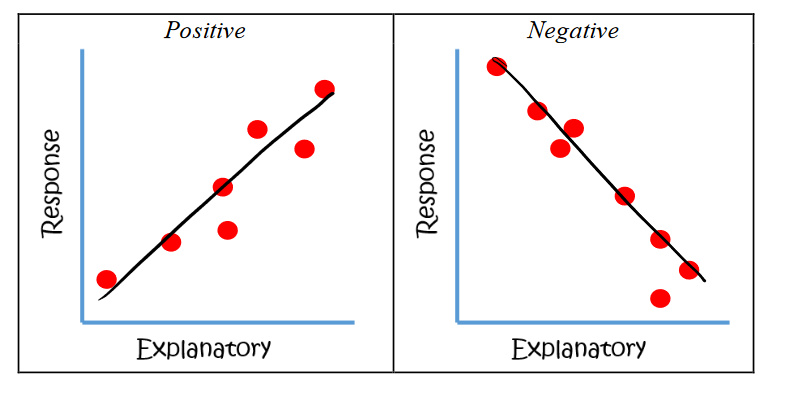
\includegraphics[width=0.8\textwidth]{2.2.3.PNG}
\end{center}

Examples of strength:
\begin{center}
    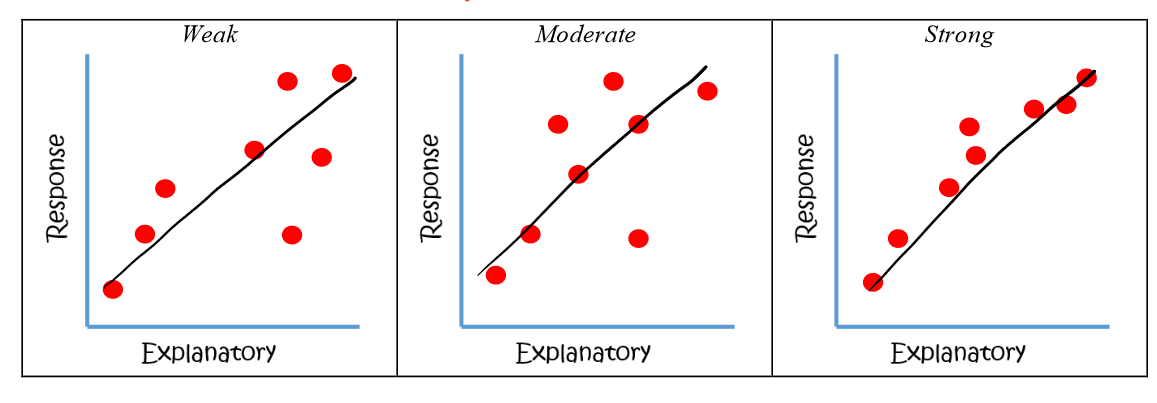
\includegraphics[width=0.8\textwidth]{2.2.4.PNG}
\end{center}

\begin{example}
    Suppose we hypothesize that the number of doctor visits a person has can be explained by the amount of cigarettes they smoke.
    So we want to see if there is a relationship between tje number of cigarettes one smokes a week and the number of times per year one visits a doctor.
    We ask 10 random people and get the following information: 
    \begin{center}
        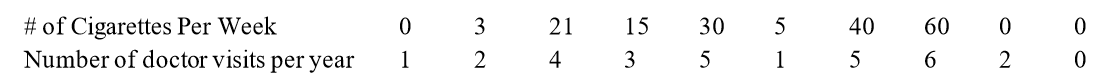
\includegraphics[width=0.8\textwidth]{2.2.5.PNG}
    \end{center}
    Creating a scatterplot gives us the following.
    \begin{center}
        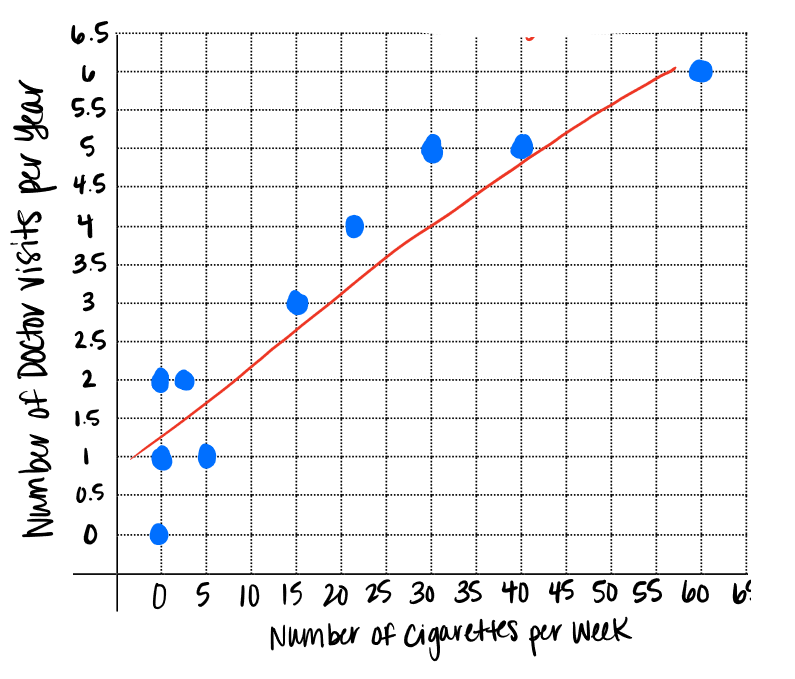
\includegraphics[width=0.8\textwidth]{2.2.6.PNG}
    \end{center}

    There is a strong, positive linear relationship between the number of cigarettes smoked per week and number of doctor visits per year.
\end{example}

If you wanted to create the previous example in a calculator, follow these steps.
\begin{enumerate}
    \item Load the $x$-values into list 1 and the $y$-values into list 2.
    \item Using StatPlot - highlight the mini-scatterplot: XList:L1 and YList:L2 
    \item Press ``graph'' but you will have to ``Zoom 9'' to fit the scatterplot on the screen 
\end{enumerate}

Unusual Features
\begin{center}
    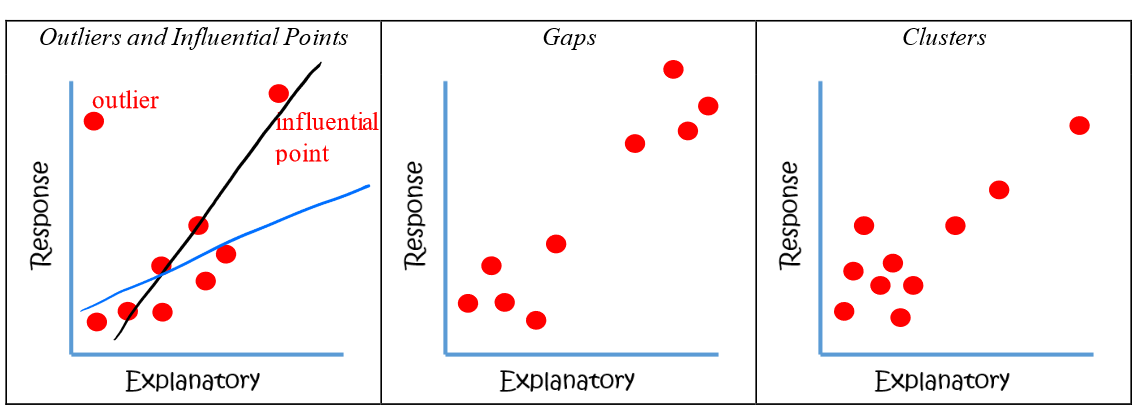
\includegraphics[width=0.8\textwidth]{2.2.7.PNG}
\end{center}

In order to strengthen the analysis when comparing two variables, we can attach a number, called the correlation coefficient ($r$), to describe the linear relationship between two variables. This number helps remove any subjectivity in reading a linear scatter plot.

The correlation measures the strength and direction of the linear relationship between two quantitative variables.

While we will never have to find correlation by hand, the formula is provided to us on the AP Statistics formula sheet. There are a few facts about the correlation that the formula can help us remember.

\[ r=\frac{1}{n-1}\sum \left(\frac{x_i-\overline{x}}{s_x}\right) \left(\frac{y_i-\overline{y}}{s_y}\right) \]
where $r$ is the correlation, $x_i$ is each x-value, $y_i$ is each y-value, $\overline{x}$ is the mean of the x values, $\overline{y}$ Is the mean of the y-values, $s_x$ is the standard deviation of x values, $s_y$ is the standard deviation of y values.

Essentially, the correlation coefficient, $r$, finds the average of the product of the standardized scores.

Correlation is a number that is between -1 and 1.
\begin{center}
    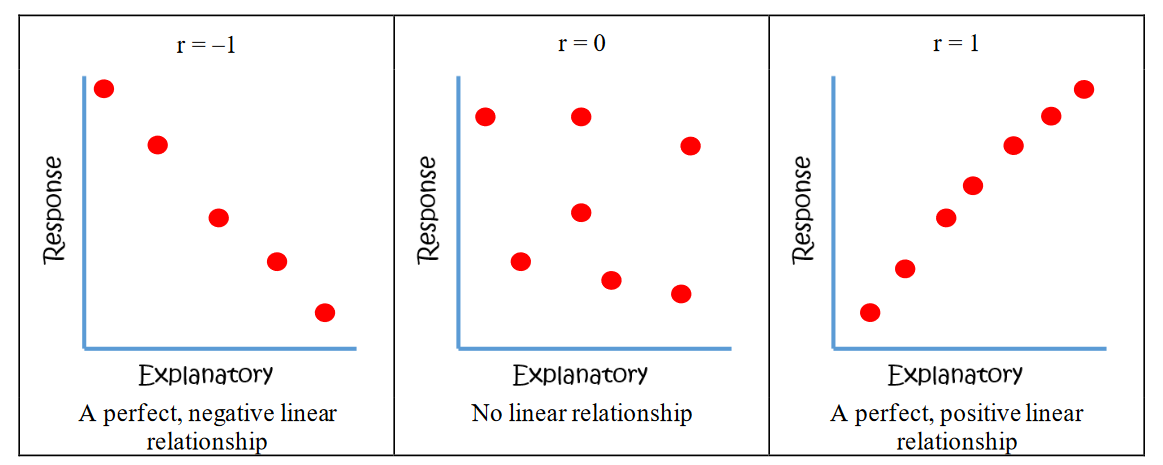
\includegraphics[width=0.8\textwidth]{2.2.8.PNG}
\end{center}

Positive correlations between 0 and 1 have varying strengths, with the strongest positive correlations being closer to 1.
\begin{center}
    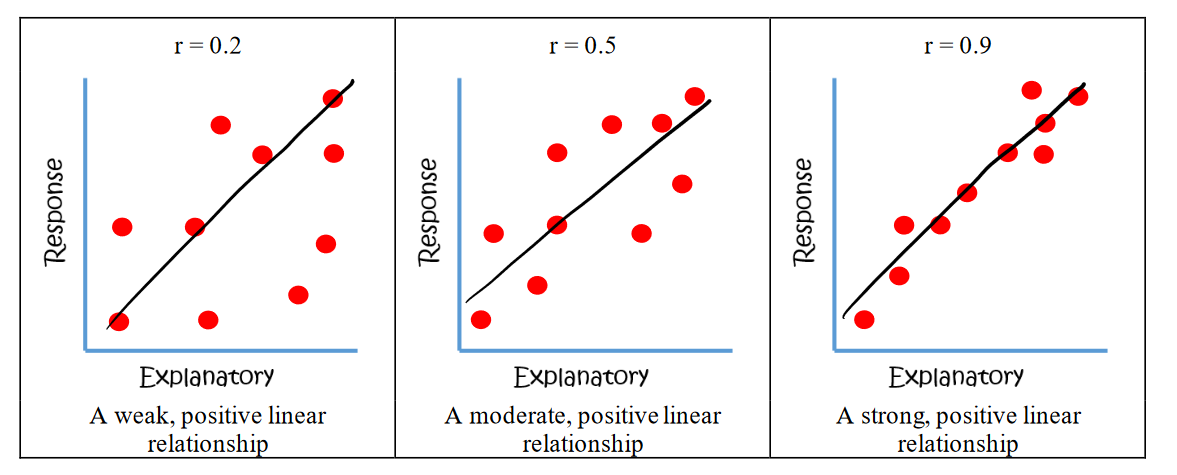
\includegraphics[width=0.8\textwidth]{2.2.9.PNG}
\end{center}

Negative correlations between -1 and 0 have varying strengths, with the strongest negative correlations being closer to -1.
\begin{center}
    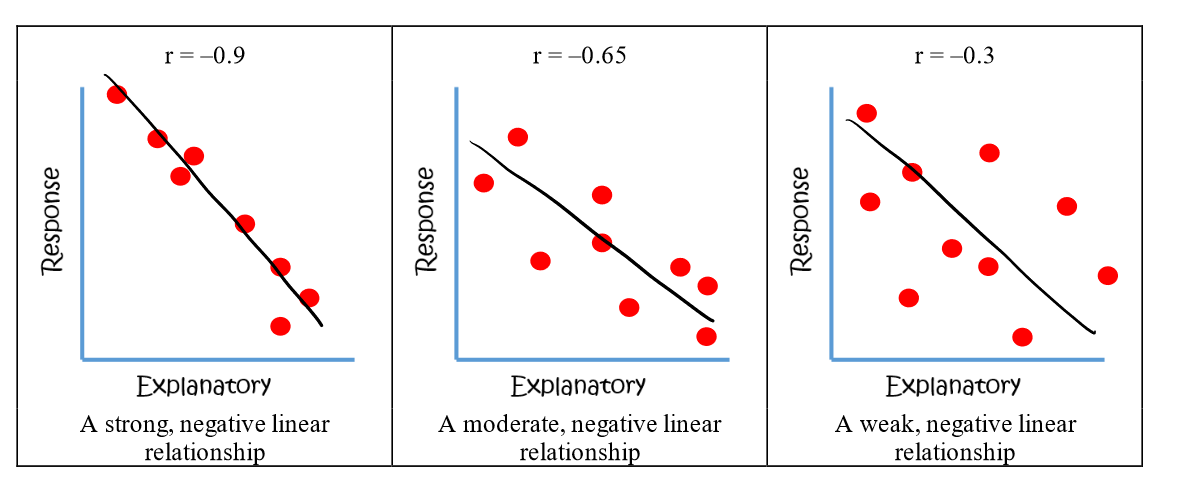
\includegraphics[width=0.8\textwidth]{2.2.10.PNG}
\end{center}

Correlation describes only linear relationships between two variables. For example, a quadratic relationship would have a correlation of 0 because it is not a linear relationship.

Correlation does not have units and changing units on either axis will not affect correlation.

If you look at the formula from above for correlation, since we are a standardizing all the $x$ and $y$ values, it does not matter what the units are. We take the product of their standardized scores.

Switching the explanatory and response variables on the axes will not change the correlation.

From the formula, this is because the order of the multiplication does not matter. Correlation makes no distinction between explanatory and response variables. It makes no difference which variable you call x and which you call y when calculating the correlation.

Correlation is very strongly affected by outliers.

Use correlation with caution when outliers appear in your scatter plot. Don't rely on correlation alone to determine the linear strength between two variables - graph a scatter plot first.

\section{Linear Regression}
Least Squares Regression or linear regressions allows you to fit a line to a scatterplot in order to be able to better interpret the relationship between two variables, as well as make predictions about our reponse variable.

The fitted line is called the line of best fit, linear regression line, or least squares regression line, (LSRL) and has an equation in a form that should look very familiar:
\[ \hat{y}=a+bx \]
where $\hat{y}$ is the predicted y-value, $x$ is the explanatory variable, $b$ is the slope, $a$ is the y-intercept.

Another way the LSRL is written is $\hat{y}=ax+b$. 

Slope is always the coefficient of $x$ and it may be called ``a'' or ``b''.

The way the line is fitted to the data is through a process called the method of least squares. The main idea behind this method is that the square of the vertical distance between each data point and the line is minimized.

\begin{itemize}
    \item If you add all of the vertical distances from the point to the line you get 0.
    \item We square each distance to make it positive, and then add it all up.
\end{itemize}

\begin{center}
    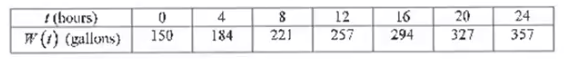
\includegraphics[width=0.8\textwidth]{2.3.1.PNG}
\end{center}

Slope: The slope of the regression line is important in the sense that it gives us the change of $y$ with respect to $x$. In order words, it gives us the amount of change in $y$ when $x$ increases by 1.

Intercept: The intercept is statistically meaningful only when $x$ can actually take values close to zero. When it does make sense to have a $x$-value of zero, the $y$-intercept is the $y$-value we would expect.

When we have a data set $(x,y)$, we can calculate the LSRL by hand or with technology.

\begin{example}
    Many schools require teachers to have evaluations done by students. A study investigated the extent to which student evaluations related to grades. Teacher evaluations and grades are both given on a scale of 100. The evaluation score (y) of a teacher from 10 of her students are given below with the average for each student (x).
    \begin{center}
        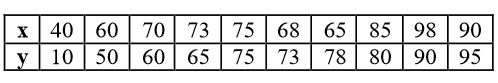
\includegraphics[width=0.8\textwidth]{2.3.2.PNG}
    \end{center}
    (a) Create the LSRL by hand.

    Step 1: Enter the data into your calculator. $x$ values go into L1 and $y$ values into L2.

    Step 2: Find the slope of your LSRL. The slope = $r\left(\frac{s_y}{s_x}\right)$. In this case, it will be 1.33.

    Step 3: Find the y-intercept of your LSRL. The y-intercept = $\overline{y}$ - slope * $\overline{x}$. In this case, the y-intercept is -28.69.

    Step 4: Create your equation: 

    $\hat{\text{teacher eval score}} = -28.69+1.33(\text{student score})$

    (b) Use your equation to predict what evaluation Mrs. H will get from a student who scored a 81.

    When you plug in 81 into the equation you made for student score, the estimated score will be 79.04.

    (c) Interpret the slope in the context of the problem.

    As student score increases by 1 point, we predict teacher eval. score to increase by 1.33 points.

    (d) Do you think student grades and evaluations students give their teachers are related? Explain.

    The correlation of 0.90 indicates a strong, positive, linear relationship between student score and TES.
\end{example}
LSRL on Calculator: There are two ways to get the line and it depends on how you like to write the line.
\begin{enumerate}
    \item Stat $\rightarrow$ Calc $\rightarrow$ 4: LinReg(ax+b)
    \item Stat $\rightarrow$ Calc $\rightarrow$ 8: LinReg(a+bx)
\end{enumerate}

Be careful when making predictions beyond what the data shows.

Extrapolation is the use of a regression line for prediction far outisde the interval of values of the explanatory variable $x$ used to obtain the line. Such predictions are not accurate.

Correlation does not imply causation. For example, there was a study that showed a strong positive linear relationship between ice cream sales and homicides in New York City. Does this mean that if we stop selling ice cream, we will have no more homicides?

Coefficient of Determination 
\begin{itemize}
    \item The strength of a prediction which uses the LSRL depends on how close the data points are to the regression line.
    \item The mathematical approach to describing this strength is via the coefficient of determination ($r^2$)
    \item The coefficient of determination ives us the proportion of variation in the values of $y$ that is explained by least-squares regression of $y$ on $x$.
    \item The coefficient of determination turns out to be the correlation coefficient squared.
\end{itemize}

In the last example, the $r$ value was 0.90. The coefficient of determination would be this number squared, so 81\%.

Whenever you use the regression line for prediction, also include a measure of how successful the regression is in explaining the reponse.

This means that 81\% of the variation in teacher evaluations can be explained by the linear relationship it has with the student class average.

Residuals 
\begin{itemize}
    \item In most cases, no line will pass exactly through all the points. This means that even if we use the LSRL to make predictions about our dependent variable, there will still be some error from the actual $y$-value.
    \item Because we use the line to predict $y$ from $x$, the prediction errors we make are errors in $y$, the vertical direction in the scatterplot.
    \item A good regression makes the vertical deviations of the points from the line as small as possible.
    \item A residual is the difference between an observed value of the response variable and the value predicted by the regression line.
    \item Residual = observed - predicted OR residResidual = $y-\hat{y}$.
    \item If the residual is positive, the observed point lies above the least squares regression line.
    \item If the residual is negative, the observed point lies below the least squares regression line.
\end{itemize}

If you add up all the residuals from your data, you will get ``0''. That is why the LSRL involves squaring the residuals then adding them up and minimizing that value.

\begin{example}
    Everyone knows that cars and trucks lose value the more they are driven. Can we predict the price of a used Ford F-150 SuperCrew 4x4 if we know how many miles it has on the odometer? A random sample of 16 used trucks was selected from autotrader.com. Here is a graph of the data.
    \begin{center}
        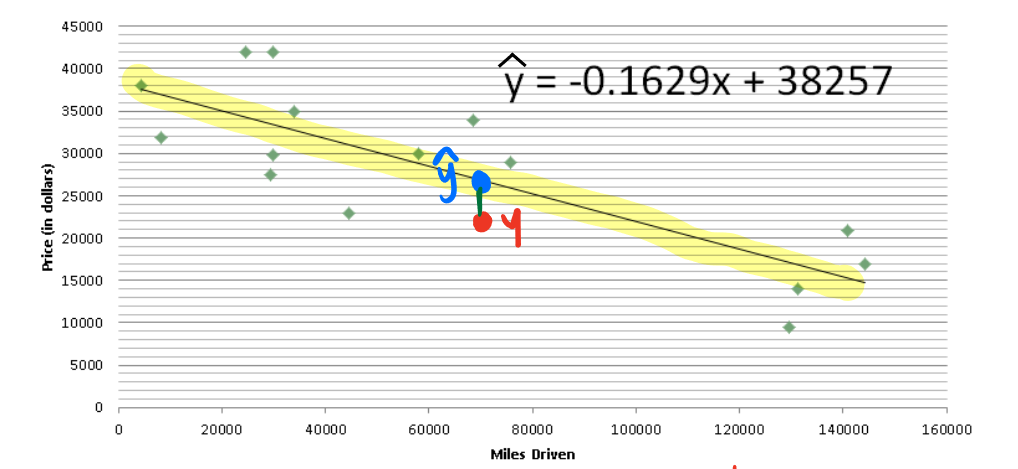
\includegraphics[width=0.8\textwidth]{2.3.3.PNG}
    \end{center}

    Find and interpret the residual for the Ford F-150 that has 70,583 miles driven and a price of \$21,994.

    Use the LSRL equation given, and we can get $\hat{y}=26759.03$. The residual is $21994-26759.03=-4765.03$.

    For a truck with 70,583 miles, our linreg overestimates the cost by \$4,765.03.
\end{example}

Residual Plots 
\begin{itemize}
    \item A residual plot makes it easy to study the residuals by plotting them against the explanatory variable.
    \item Residual plots help us assess whether a linear model is appropriate.
    \item In the truck example, if we calculate all the residuals for each plot, we can then plot the miles driven vs. residuals.
\end{itemize}
\begin{center}
    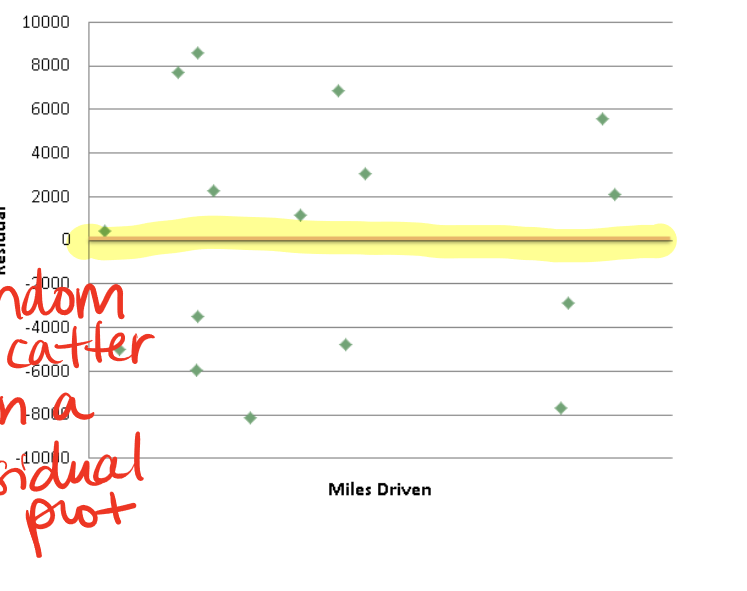
\includegraphics[width=0.8\textwidth]{2.3.4.PNG}
\end{center}
\begin{itemize}
    \item Essentially, a residual plot turns the regression line horizontal.
    \item Residual plots magnify the deviations of points from a line.
    \item This makes it easier to see an unusual pattern, so it helps us determine if a linear model is appropriate.
\end{itemize}

When an obvious pattern exists in a residual plot, the model we are using is not appropriate. For example 
\begin{center}
    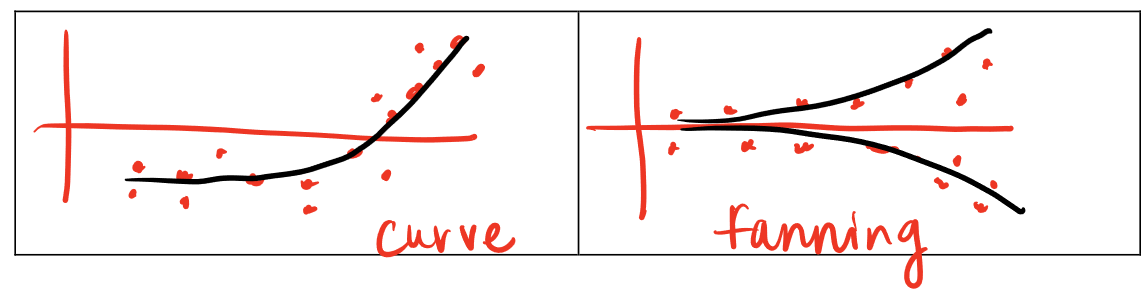
\includegraphics[width=0.8\textwidth]{2.3.5.PNG}
\end{center}

The TI-83/84 will generate a complete list of residuals when you perform a LinReg. They are stored in a list called RESID which can be found in the LIST menu. RESID stores only the current set 
of residuals. That is, a new set of residuals is stored in RESID each time you perform a new regression.

In order to draw a residual plot on the TI-83/84, first enter your data and perform a LinReg. Next, create a STAT PLOT where XList is L1 and YList is RESID (get this by pressing 2nd $\rightarrow$ STAT $\rightarrow$ 9:)
\section{Influential Points and Departure from Linearity}
Sometimes called ``MiniTab'', computer output on the AP exam is a quick way to give statistical information on linear regression. The key is to remember what all the information stands for.
\begin{center}
    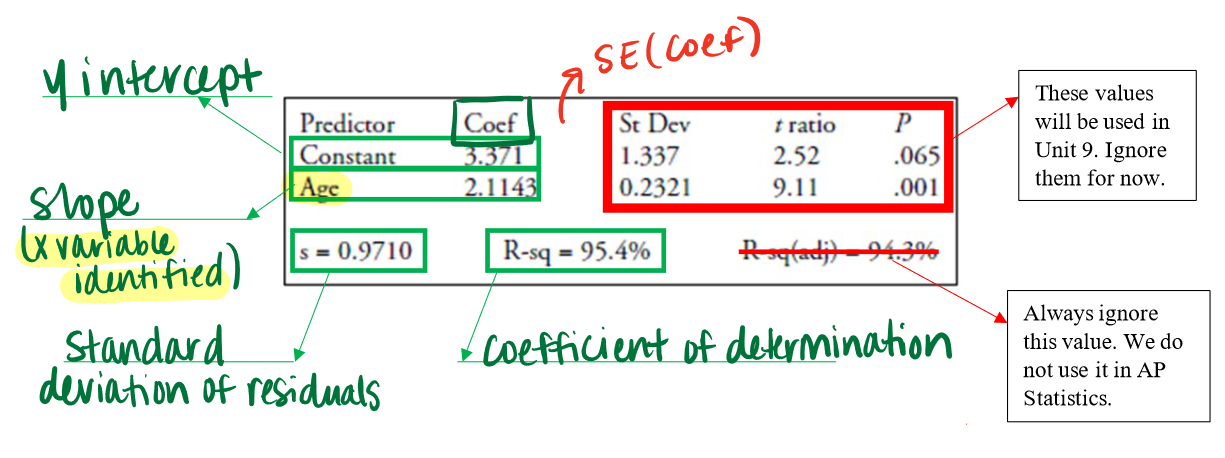
\includegraphics[width=0.8\textwidth]{2.4.1.PNG}
\end{center}
Using the above information, we can also get the following:

LSRL: $\hat{y}=3.371+2.1143$(age) and $r=\sqrt{0.954}=0.9767$.

The standard deviation of the residuals (``$s$'') will be used more in Unit 9, but we can interpret it here. This value gives the approximate size of a ``typical'' prediction error (residual). Larger values of 
``$s$'' means our line is expected to give larger residuals. The units for the standard deviation of residuals is the same of the residuals (and of the $y$-values). So it depends on the data for what is considered a ``large'' residual error.

For example, if ``$s$'' was 100, that would be a large value if our $y$-value was trying to predict age in years but it would be a small residual if we were trying to predict age in seconds. Context is important when interpreting this value.

An influential point in a data set, is a point that has leverage on the correlation and regression line. In other words, when removed, this point changes the regression line substantially. 
An influential point might be considered an outlier if it does not fit with the overall pattern of the data, but an influential point might also fit the data, but change the regression line and/or correlation significantly when removed.
\begin{example}
    Here is a set of hypothetical data and its scatterplot.
    \begin{center}
        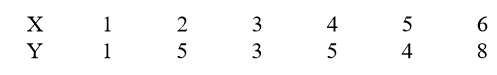
\includegraphics[width=0.8\textwidth]{2.4.3.PNG}
    \end{center}
    \begin{center}
        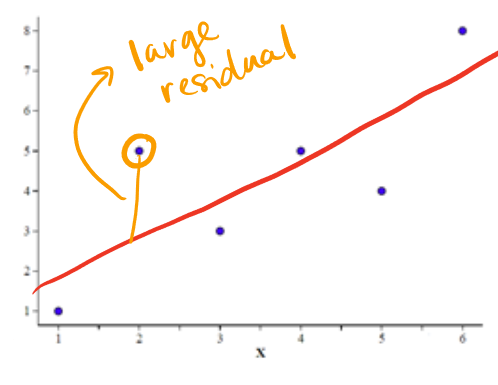
\includegraphics[width=0.8\textwidth]{2.4.2.PNG}
    \end{center}

    The LSRL: $\hat{y}=.9333+.9714x$ and the $r$ is $.777$.

    Suppose we removed $(2,5)$. The point is not considered an outlier because it fits the rest of the data, but we will examine the impact on the LSRL and correlation to see that it is influential.

    The LSRL becomes $\hat{y}=-0.473+1.2297x$ and $r=0.914$.

    The slope increased singe that point has leverage and was pulling our LSRL towards it.

    The y-intercept decreased since the slope increased, it moved the $y$-intercept lower.

    The correlation ($r$) also increased. The point $(2,5)$ is not considered an outlier but since it had a large residual originally, removing it made teh LSRL ``fit'' better.
\end{example}

The AP Statistics course deals only with two-variable data that can be modeled by a line OR nonlinear two-variable data that can be transformed in such a way that the 
transformed data can be modeled by a line.

To know what transformation to use, graph the data first. If the scatterplot does not show a linear pattern, or the residual plot pattern is not random, consider a transformation.

You can transform the independent variable, dependent variable, or both. There are a wide range of transformations you can do, but the AP exam will keep it simple. Here is an example of one of the most common transformations you will encounter.

\begin{example}
    The number of a certain type of bacteria present (in thousands) after a certain number of hours is given in the following table.
    \[ \begin{tabular}{c|c}
        Hours & Numbers \\
        \hline 
        1.0 & 1.8\\ 
        1.5 & 2.4\\
        2.0 & 3.1\\
        2.5&4.3\\
        3.0&5.8\\
        3.5&8.0\\
        4.0&10.6\\
        4.5&14.0\\
        5.0&18.0
    \end{tabular}\]

    The following are the scatterplot and the residual plot.
    \begin{center}
        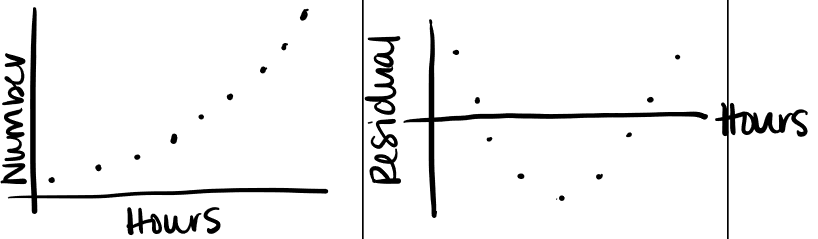
\includegraphics[width=0.8\textwidth]{2.4.4.PNG}
    \end{center}

    A linear model is not appropriate here because the scatterplot shows an exponential form and the residual plot is curved.
    \begin{itemize}
        \item What parent function does this scatterplot look like? Exponential!
        \item How do we undo exponents? Logs
        \item For this problem the natural logarithm will be the best way to transform the data to achieve linearity.
        \item On the AP exam, to save time, if you needed to do this by hand, they would tell you the transformation.
    \end{itemize}

    The data is now 
    \[ \begin{tabular}{c|c|c}
        Hours & Numbers & LN(Number) \\\hline 
        1.0 & 1.8&0.59\\ 
        1.5 & 2.4&0.88\\
        2.0 & 3.1&1.13\\
        2.5&4.3&1.46\\
        3.0&5.8&1.76\\
        3.5&8.0&2.08\\
        4.0&10.6&2.36\\
        4.5&14.0&2.64\\
        5.0&18.0&2.89
    \end{tabular}\]

    The scatterplot and residual plot:
    \begin{center}
        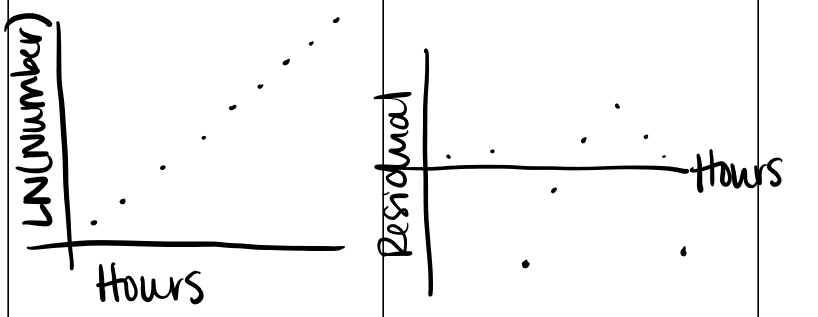
\includegraphics[width=0.8\textwidth]{2.4.5.PNG}
    \end{center}

    This is a better model for linear regression because the scatterplot shows a straight-line pattern and the residual plot shows random scatter.

    The regression equation for the transformed data is ln($\hat{\text{number}}$) = $-0.0047+.586(\text{hours})$. 

    If we wanted to find the predicted quantity of bacteria after 3.75 hours, we can plug that number in and get 8,906.3 bacteria as the answer.
\end{example}

There are many types of transformations avaliable and you can even get really crafty and add in some constants.

For AP Statistics, we keep it simple. Here are some common patterns.
\begin{center}
    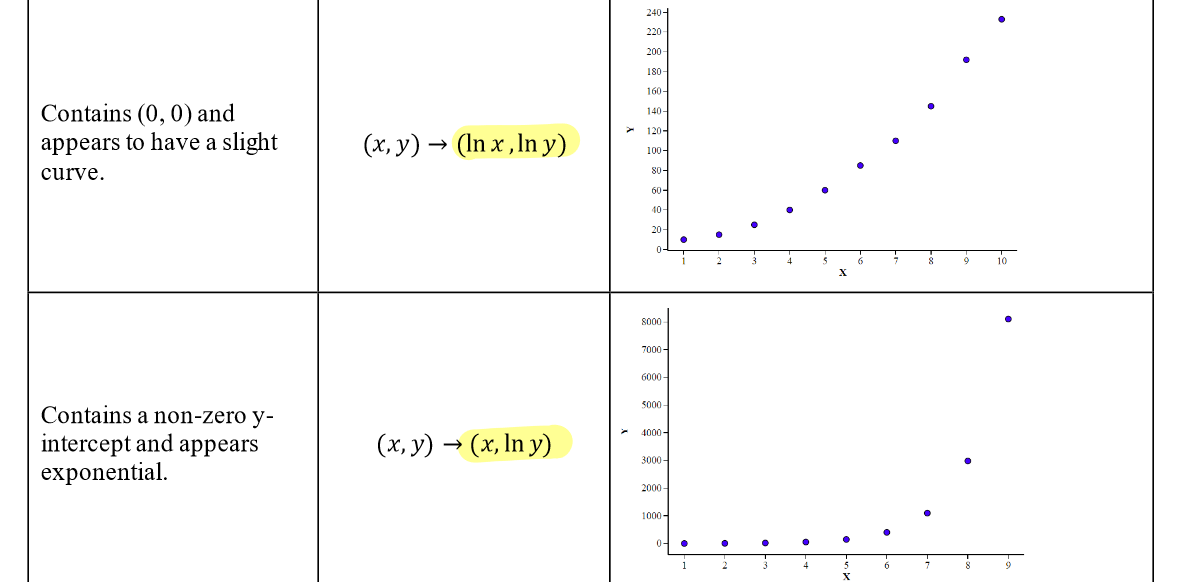
\includegraphics[width=0.8\textwidth]{2.4.6.PNG}
\end{center}
\begin{center}
    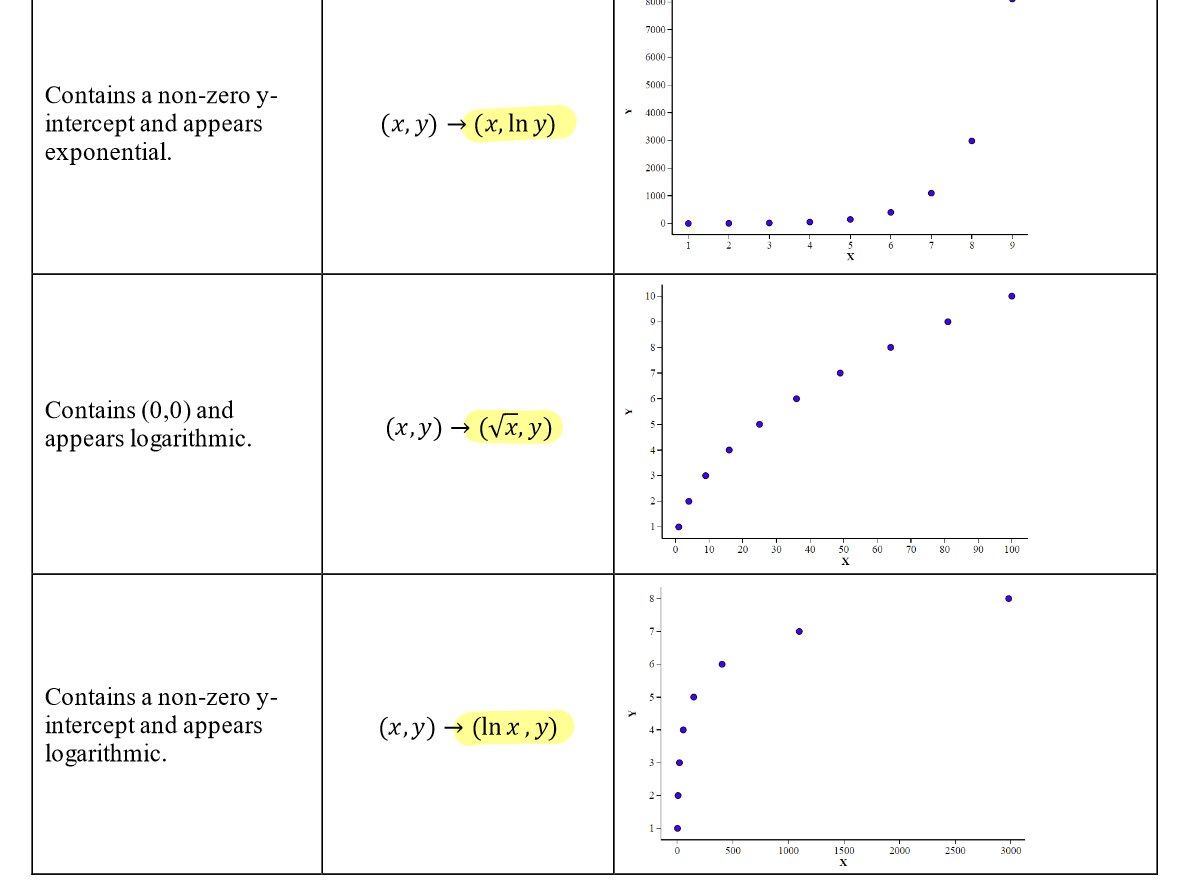
\includegraphics[width=0.8\textwidth]{2.4.7.PNG}
\end{center}
To test and see which model would be appropriate, you would compare the scatterplots, $r$ and $r^2$, and the residual plots of both the original and transformed data.
\end{document}